
For our experiments we chose to use WebQuestions dataset, which become a standard benchmark for KBQA in recent years and a lot of work has been published on this dataset.
The dataset used Freebase as a KB of choice, therefore our system is based on this knowledge base despite the fact that its support has been shut down.
This means that the KB will no longer be updated, but the data is publicly available.

The overall architecture of the our model is presented on Figure \ref{fig:model}, and it's based on a model proposed in \cite{ACCU:2015}.
We will first describe the baseline system and then present our way of utilizing unstructured text resources on different stages of the QA process.
As an example we will take one of the questions from the WebQuestions dataset: \emph{Who is the woman that john edwards had an affair with?}.

\begin{figure*}[t]
\centering
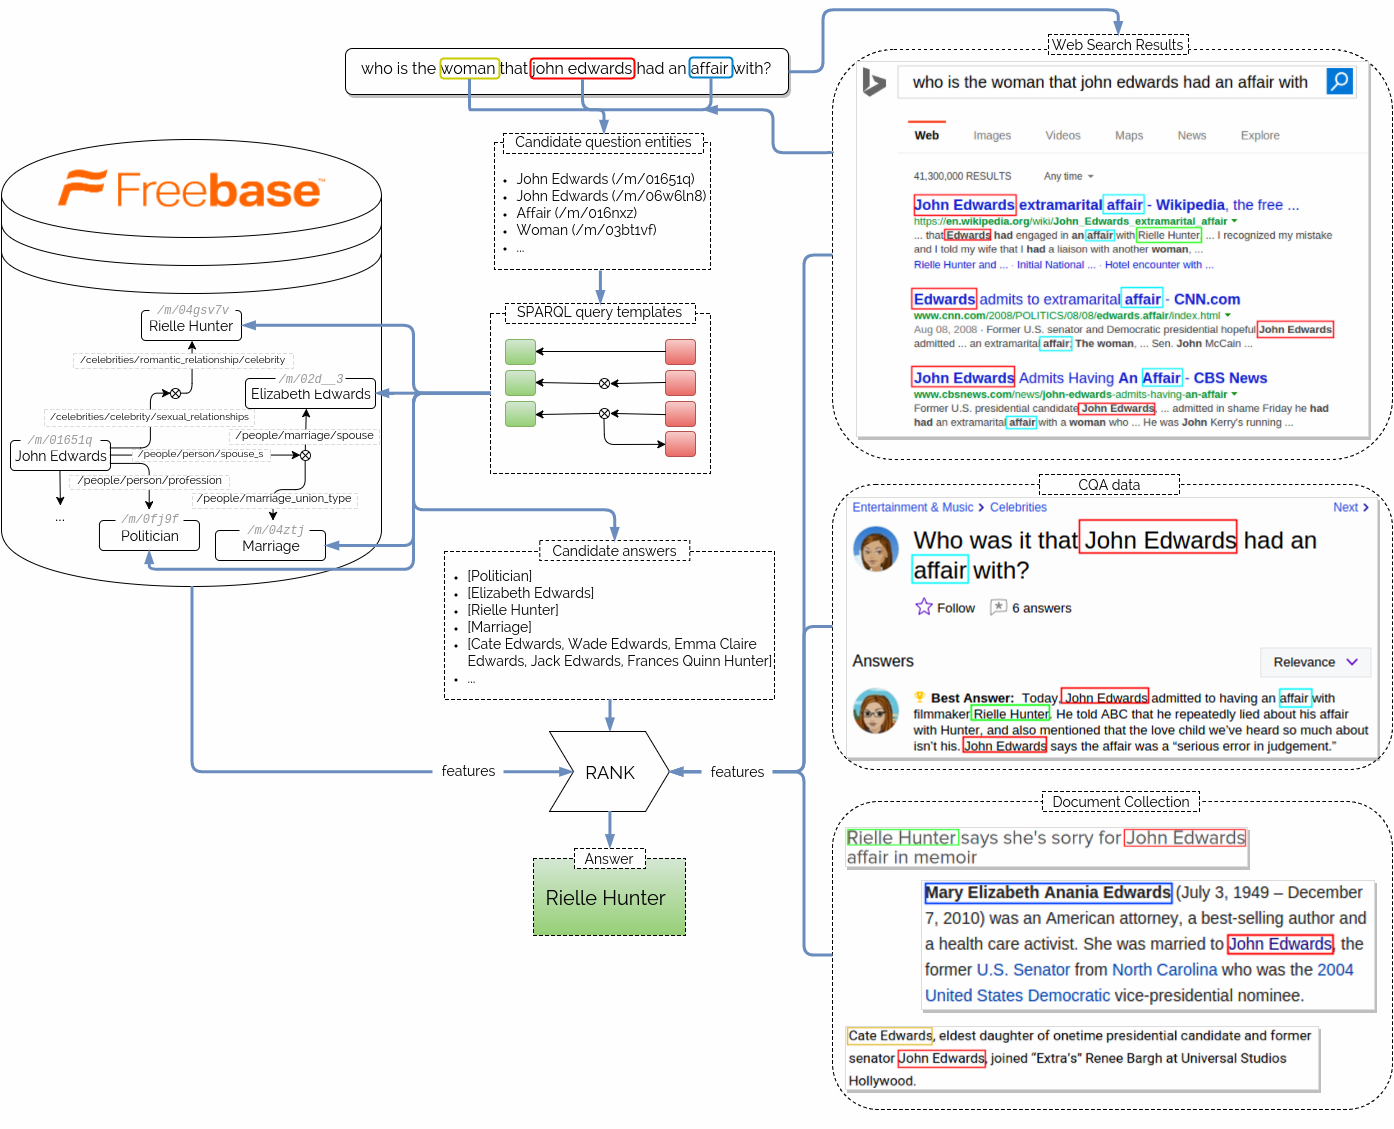
\includegraphics[width=\textwidth]{img/Text2KB_model}
\caption{The architecture of our Text2KB Question Answering system}
\label{fig:model}
\end{figure*}

\subsection{Baseline method}

The baseline system starts answering a question by \textbf{identifying KB entities} that are mentioned in the question.
In our example, entity John Edwards (/m/01651q)\footnote{This is an identifier of the entity in Freebase} is the main question entity.
However, Freebase contains millions of entities and it's often hard to identify the main ones (\eg Woman and Affair are also present in Freebase as entities) or to disambiguate and choose between John Edwards the politician (/m/01641q) and John Edwards the American sports car racing driver (/m/06zs089) and many other John Edwards' present in the KB.
There is even an entity /m/0c0n01x with the name ``had an affair with''.
The baseline system considers all spans of terms under certain conditions on POS tags and use a dictionary of names, aliases and anchor tests \cite{SPITKOVSKY12.266} to map phrases to potential entities.
Each candidate entity mention is scored and disambiguation is postponed to later stages.

After a set of candidate mentions is built, the system explores the neighborhood of the entities in the knowledge base by \textbf{matching a set of query templates} to the question.
Each template has an entity and a relation placeholders and correspond to a candidate query which can be executed against the KB and return an answer.
The baseline system uses 3 templates:
\begin{enumerate}
\item $[$question entity$]$ $\rightarrow$ $[$relation$]$ $\rightarrow$ $[$answer entity$]$
\item $[$question entity$]$ $\rightarrow$ $[$relation 1$]$ $\rightarrow$ $[$mediator node$]$\\
$[$mediator node$]$ $\rightarrow$ $[$relation 2$]$ $\rightarrow$ $[$answer entity$]$
\item $[$question entity 1$]$ $\rightarrow$ $[$relation 1$]$ $\rightarrow$ $[$mediator node$]$\\
$[$mediator node$]$ $\rightarrow$ $[$relation 2$]$ $\rightarrow$ $[$question entity 2$]$
$[$mediator node$]$ $\rightarrow$ $[$relation 3$]$ $\rightarrow$ $[$answer entity 3$]$
\end{enumerate}

Each query candidate is matched against the tokens in the question via names of relations in the KB, words learned through distant supervision and word mappings learned during training.

The last stage of the question answering process is query candidates ranking.
A random forest model is trained to rank query candidate given a set of features generated for query candidates and corresponding entity mentions.


\subsubsection{Extensions}
We implemented a couple of extensions of the baseline system.

\begin{itemize}
\item date range based filters
\item notable types based filters
\item notable types based model, used as a feature
\end{itemize}

\subsection{Unstructured text data for KBQA}

\subsubsection{Text data in KB}
We use entity descriptions to generate a set of features for candidate answers.
Description of entity in the knowledge base was found useful for question answering \cite{Sun:2015:ODQ:2736277.2741651}.
Therefore, we decided to use it as well.

Analogously, we can use entity Wikipedia profile pages.

\subsubsection{Web search results}

Traditional text-based question answering systems usually retrieve text passages relevant to the question from a large collection of documents, \eg the internet.
The same information in a large collection appears many times and often in it is expressed in different ways.
Question answering benefit from this redundancy \cite{Lin:2007:EPU:1229179.1229180} as it increases the chances of good lexical match between question and answer sentences, and makes some simple counting-based techniques quite effective \cite{brill2002analysis}.
Therefore, it's reasonable to assume that these ideas can be adopted for knowledge base question answering.

Our model issues the question as a query to a web search engine\footnote{https://datamarket.azure.com/dataset/bing/search} and extract top 10 results, \ie search snippets and corresponding documents.
Next, the system identifies KB entity mentions in both snippets and documents texts using the same method as used for question processing.
We use these data in two different ways: to extend the set of question entities and to generate features for candidate answer ranking.

\textbf{Question entity identification}.
Question test is often quite short, may contain typos and other problems, that complicate identification of question entities.
Entity detection is a crucial step in the process, because it makes it impossible to generate the correct answer candidate.
By retrieving relevant text documents it is possible to improve entity identification, as demonstrated (\cite{SMAPH_ERD:2014}) by the results of the short track in Entity Recognition and Disambiguation Challenge 2014\footnote{http://web-ngram.research.microsoft.com/ERD2014/}. 
For example, one of the questions, for which the baseline system were unable to find the correct question entity mention is \emph{``what year did tut became king?''}.
However, search results for this question (Figure \ref{fig:web_search_entitylink}) mentions the full name of the entity ``Tutankhamun'' and ``King Tut'' multiple times, which can be a good signal to add this entity to the list of detected question entities.

\begin{figure}
\centering
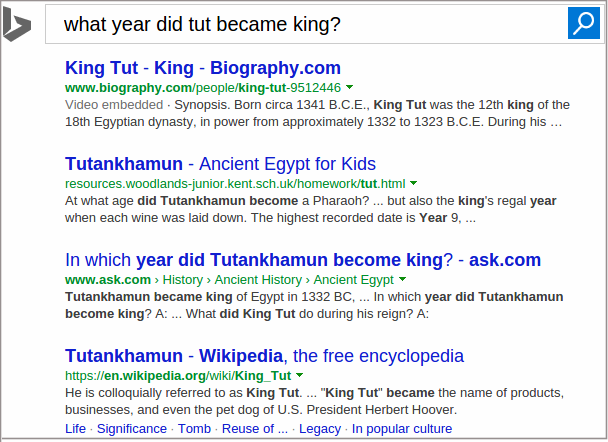
\includegraphics[width=0.5\textwidth]{img/web_search_entitylink}
\caption{Search results for the question ``what year did tut became king?''}
\label{fig:web_search_entitylink}
\end{figure}

In our system, Text2KB, we follow the following procedure to extend a set of identified KB entities identified from the question:
\begin{enumerate}
\item Detect entities mentioned in search result snippets and titles
\item An entity is added to the list of question entities if 
$$\max_{m_t \in M\backslash Stp, q_t \in Q\backslash Stp} dist(m_t, q_t) \geq 0.8$$
Here $M$ is a set of entity mention tokens, $Q$ - set of question tokens, dist() - text edit distance (we used Jaro-Winkler distance), and Stp is a set of stopwords.
\item For each question entity we count the number of mentions in search titles and snippets and use this information as a feature for answer candidate ranking.
\end{enumerate}

\textbf{Answer candidate features}.
Despite being useful for question entity identification, search results often contain the answer to the given question, \eg on Figure \ref{fig:web_search_entitylink} multiple snippets mention the date when Tutankhamun became the king.
Therefore, we use text of search results titles, snippets and documents to generate features for candidate answer ranking.
More specifically Text2KB computes the following:
\begin{enumerate}
\item Identify entities in search results titles, snippets and documents
\item Combine texts of all search result documents to form a single text (with entities identified)
\item Represent each snippet (which includes title), document and combined document as a two separate TF-IDF vectors: vector of term occurrences, vector of entity occurrences\footnote{We used Google n-grams corpus to approximate terms IDF and ClueWeb FACC entity annotations (http://lemurproject.org/clueweb09/FACC1/) to compute entity IDFs}
\item Each answer candidate is also represented as TF-IDF vectors of terms (from entity names) and entities
\item Compute cosine similarity between answer vectors and snippets, documents and combined document vectors and use maximum and average cosine similarities as features for candidate ranking.
\end{enumerate}

\subsubsection{Community Question Answering data}

Questions and corresponding answers are often expressed differently and researchers in question answering studied different ways to bridge this lexical gap, \eg using translation models \cite{Murdock:2005:TMS:1220575.1220661} and distributional semantics \cite{yu2014deep}.

Modern Knowledge base question answering systems are typically trained from question-answer pairs \cite{Berant:EMNLP13}.
Specifying correct answer entities requires much less effort than labeling with correct logical forms, but this manual process still limits the size of training datasets.

On the other hand community question answering (CQA) websites contain millions of question-answer pairs and therefore the idea of adapting this data for model training looks very attractive.
However, majority questions of CQA websites aren't factoid and even for factoid question the answer provided is typically verbose and we need to detect which (if any) of the mentioned entities actually answers the question.



Using a collection of question-answer pairs from Yahoo! Answers we annotated questions and answers with entities and relations between pairs of entities.
This approach follows distant supervision approach for relation extraction \cite{savenkov-EtAl:2015:SRW}.
Pairs of question words and relations are used to generate features.

\subsubsection{Entity-linked collection of documents}
We take ClueWeb12 and use existing entity links generated by Google to build an index from entity pair to phrases, that occur around these entities in the collection.
This data is used to generate features for candidates.

\subsubsection{Wikipedia profile}
It would be nice to have Wikipedia pages for entities and use something like SDM score or something else as feature.